\chapter{Quantum Graph Neural Networks for Molecular Property Prediction}

\section*{Abstract}

Hydrogen research, particularly in the fields of energy storage and catalysis, hinges on a deep understanding of molecular interactions and properties. The surface area of molecules is a crucial parameter influencing hydrogen adsorption and catalytic efficiency. Traditional computational methods for predicting molecular surface areas, while effective, face challenges in terms of computational complexity and accuracy when dealing with large and complex molecular structures. The accurate prediction of molecular surface area is paramount in optimizing hydrogen storage and catalysis processes. Conventional computational models, primarily based on classical algorithms, struggle with the vast complexity and quantum nature of molecular systems. This gap necessitates a novel approach that can handle the quantum mechanical properties inherent in molecules more naturally and efficiently.

\textit{\textbf{Keywords:} quantum machine learning, quantum graph neural networks, hydrogen research, potential energy surface prediction}

\section{Introduction}

\begin{figure}[h!]
    \begin{subfigure}{.5\textwidth}
     \captionsetup{justification=centering}
      \centering
      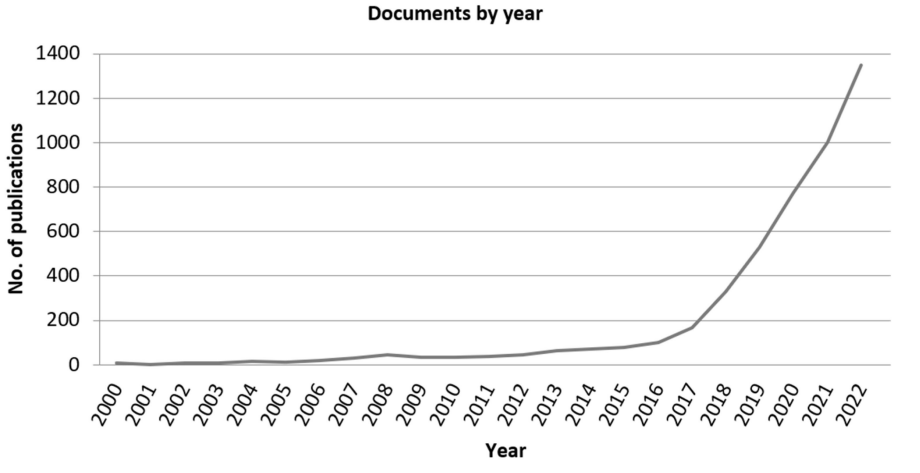
\includegraphics[width=.8\linewidth]{QML-Documents.png}
      \caption{Number of documents released per year in the field of QML}
      \label{fig:sfig1}
    \end{subfigure}%
    \begin{subfigure}{.5\textwidth}
      \centering
      \captionsetup{justification=centering}
      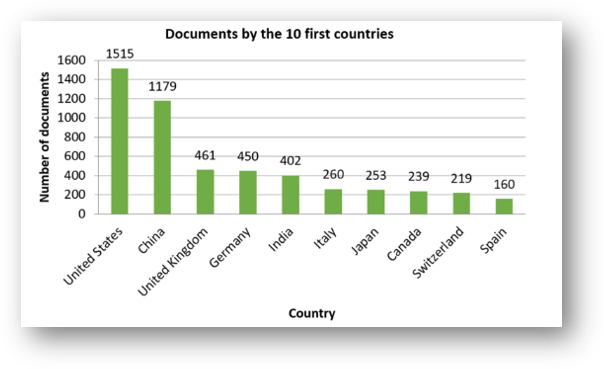
\includegraphics[width=.8\linewidth]{QML-countries..png}
      \caption{Number of documents released per country in the field of QML}
      \label{fig:sfig2}
    \end{subfigure}
    \caption[Results of QML-Literature-Overview from Tychola et al. 2023 (excerpt)]{\label{img:tychola} Results of QML-Literature-Overview from Tychola et al. 2023 \cite{Tychola_Kalampokas_Papakostas_2023} (excerpt)}
    \end{figure}

While there is growing research on the application of quantum computing in various domains, including chemistry and materials science, the specific application of QGCNNs for predicting molecular surface area in hydrogen research remains underexplored. This presents an opportunity to bridge the gap between quantum computing and molecular science, particularly in the context of hydrogen storage and catalysis. Recent advancements in quantum computing offer promising avenues for addressing complex problems in molecular sciences. Quantum Graph Convolutional Neural Networks (QGCNNs) have emerged as a potential tool for processing graph-structured data, which is naturally suited for molecular representations (Bronstein et al., 2017). The application of quantum computing in neural networks has shown significant improvements in handling high-dimensional data and complex interactions (Biamonte et al., 2017). Moreover, the representation of molecules as graphs aligns well with the capabilities of GNNs in capturing the intricate relationships and features within such structures (Duvenaud et al., 2015). The accurate prediction of molecular surface area is paramount in optimizing hydrogen storage and catalysis processes. Conventional computational models, primarily based on classical algorithms, struggle with the vast complexity and quantum nature of molecular systems. This gap necessitates a novel approach that can handle the quantum mechanical properties inherent in molecules more naturally and efficiently.

In order to solve the presented problem, the following research question and sub-questions are created: 
\begin{center}
    \textit{"How can a Quantum Graph Neural Network for the prediction of molecular properties be developed?"} \\
\end{center}
Q1: \textit{How do Quantum Graph Neural Networks work?} \\
Q2: \textit{How must molecular data be processed to be used with a quantum computer?} \\
Q2: \textit{How does the performance compare to classical Graph Neural Networks?} \\

The goal of this paper is to develop an understanding of quantum graph neural networks and how they work. Besides, in the scope of this paper, an understanding of the prediction of potential energy is created. Based on this procedure, the analysis of different foundation papers  will show how a quantum graph neural network can be developed. In summary, to answer the developed research question and sub-questions, the following artifacts will be created as part of the research: 

\begin{itemize}
    \item foundation paper analysis of different papers in the context of quantum graph neural networks
    \item requirement analysis for prediction of a quantum graph neural network for the prediction of molecular properties based on the analysis of the foundation papers
    \item attempt to develop a quantum graph neural network based on the conducted requirement analysis
\end{itemize}  

The structure of this paper is as followed: first, the scientific foundations and theoretical background are discussed. Then the research methodology is presented in detail. Based on this, the findings and their results are presented and then discussed. Finally, a conclusion and discussion of the results is provided, as well as an overview of possible research topics based on this work.   

\section{Theoretical Background}
\subsection{Quantum Computing}
In order to understand the fundamentals of quantum computing, it is first necessary to explain the basic building blocks of quantum computing. These are also known as quantum bits, quantum gates and quantum circuits, and are explained in the following. In quantum computing, quantum bits, or qubits, are the basic units of information. Unlike classical bits, which can only take the states 0 or 1, qubits operate according to the principles of quantum mechanics, which allows them to take both states simultaneously. This overlapping is called superposition and enables an exponential increase in information density. \cite{claudino2022basics} Quantum gates are the building blocks for quantum circuits and perform operations on qubits. They are the analogue of logic gates in classical computer science, but with the difference that quantum gates perform continuous transformations, also known as unitary transformations, which change the superposition states of the qubits. An example of single quantum gates are Pauli rotation gates. These are applied by extracting the exponentials of the Pauli operator.

\begin{table}[h!]
    \centering
    \captionsetup{justification=centering}
    \begin{tabular}{ccc}
    \hline
    \textbf{Gate} & \textbf{Matrix Representation} \\ 
    \hline
    $R_x$ gate & $\begin{pmatrix} \cos\frac{\theta}{2} & -i\sin\frac{\theta}{2} \\ -i\sin\frac{\theta}{2} & \cos\frac{\theta}{2} \end{pmatrix}$ \\ 
    $R_y$ gate & $\begin{pmatrix} \cos\frac{\theta}{2} & -\sin\frac{\theta}{2} \\ \sin\frac{\theta}{2} & \cos\frac{\theta}{2} \end{pmatrix}$ \\ 
    $R_z$ gate & $\begin{pmatrix} e^{-i\frac{\theta}{2}} & 0 \\ 0 & e^{i\frac{\theta}{2}} \end{pmatrix}$ \\ 
    \hline
    \end{tabular}
    \caption[Pauli-rotation gates according to Zheng et al. 2021]{\label{tab:pauligates} Pauli-rotation gates according to Zheng et al. 2021 \cite{zheng2021quantum}}
\end{table}

There are also two-bit gates, which perform operations on two qubits and thus logically link them together. One example of this is the CNOT gate, which is used frequently in the field of quantum computing. \cite{zheng2021quantum} Quantum circuits are a combination of the previously introduced quantum gates and qubits. This is a specific sequence of quantum gates that are applied to a specific number of qubits in order to perform complex calculations. A quantum circuit is always designed for a specific application. This enables a variety of specific applications such as the simulation of molecular interactions. \cite{claudino2022basics}

\subsection{Quantum Graph Neural Networks}
\subsection{Potential Energy Prediction}
The potential energy surface (PES), in the context of molecules and atoms, describes the energy of a molecule in regard to certain parameters, e.g. to the position of its atoms.    
Predicting the potential energy surface of atoms is a task in computational chemistry and materials science. It gives information about the stability and properties of molecules and materials \cite{liu_computational_2023}. This is helpful when to decide whether materials can be used to enable efficient catalytic processes in the field of hydrogen production \cite{chen_waste-derived_2023}. 

\section{Research Methodology}

First, the given problem of constructing QGNNs for the prediction of molecular properties was investigated. For this purpose, an initial investigation of the literature took place and the topic was explored. This is followed by the definitions of the research questions as well as the sub-questions and the delineation of the research topic. \\

\begin{figure}[h!]
    \centering
    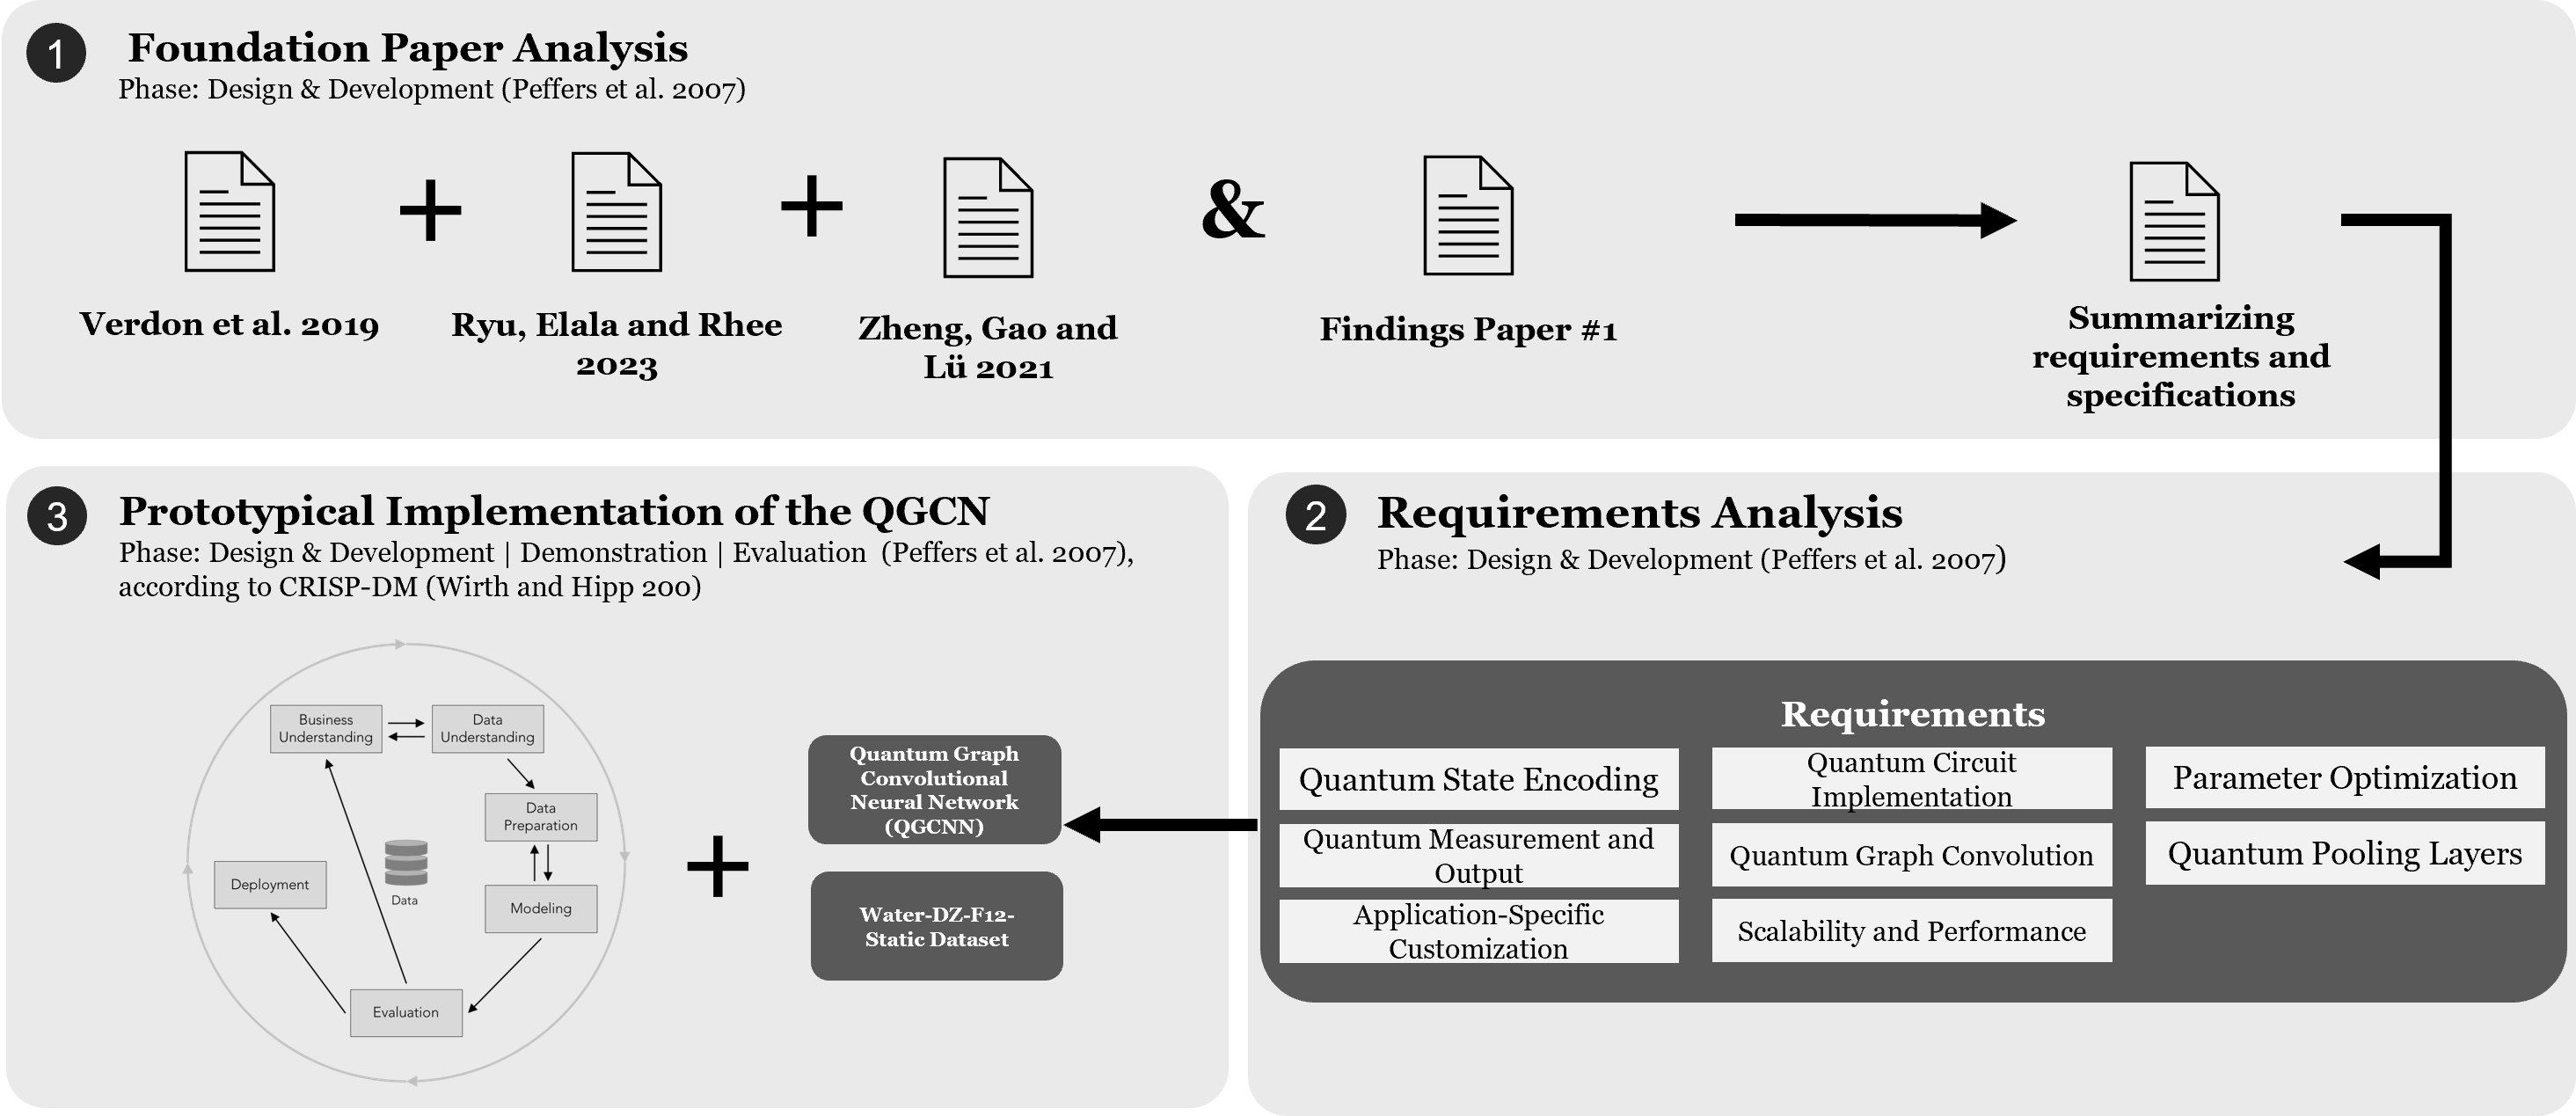
\includegraphics[width=\textwidth]{05_paper02RM.png}
    \caption[Overview of the conducted research process]{\label{img:paper02rm}{Overview of the conducted research process}}
    \end{figure} 

Three foundation papers were then analyzed to investigate different approaches to the development of QGNNs and to identify a possible approach to the development of a QGNN for the prediction of molecular properties. Together with the results of the first paper of this thesis and the results of the foundation paper analysis, requirements for the QGNN to be developed are defined. Using these requirements, this paper will attempt to develop a prototype QGNN. This will enable the prediction of molecular properties using QGNNs to be tested and a comparison to classical GNNs to be made.  For a better structure and traceability of the procedure, the exact research process is shown in Figure \ref{img:paper02rm} on the previous page, which is described in detail in the following section. \\

The \textbf{first step} was to analyze the foundation papers. The papers by Verdon et al. \cite{verdon_quantum_2019}, Zheng, Gao and Lü \cite{zheng2021quantum} and the paper by Ryu, Elala and Rhee \cite{ryu2023quantum} were used. Since the literature on QGNNs is limited to a very small number of papers, a structured literature analysis is not useful in this case. Accordingly, various literature databases were searched for literature on QGNNs and the papers most relevant to the topic of this thesis were selected for the foundation paper analysis. The results of the analysis of these three papers were combined with the results of the first paper of this thesis and summarized for the next step of the conducted research process. \\

In the \textbf{second step},  a requirements analysis was carried out based on the results of the foundation paper analysis. A total of 11 different requirements were identified for the QGNN to be developed. Basically, these requirements can be divided into two categories: "data preparation" and "architecture of the QGNN". The results of this requirements analysis are discussed in more detail in Section \ref{subsec:requirements}. \\

The \textbf{third step} covers the prototypical implementation of the QGNN for the prediction of molecular properties. Based on the previously identified requirements, an attempt was made to implement a QGNN capable of predicting the potential energy surface using the water data set mentioned in the first paper of this thesis. Similar to the first paper, the implementation followed the structured procedure of CRISP-DM \cite{wirth2000crisp} and is explained in Section \ref{subsec:qgnndevelopment} of this thesis. Although the QGNN could not be implemented completely successfully, the development still provides interesting insights and further work can be based on the findings of this paper.

\section{Findings}
In this section, the results and findings are presented and discussed in detail. Especially the literature review and the prototypical implementation of the GNN for the prediction of potential energy will be considered. 

\section{Findings}
\subsection{Foundation Paper}
\subsection{Requirement Analysis}
\begin{figure}[h!]
    \centering
    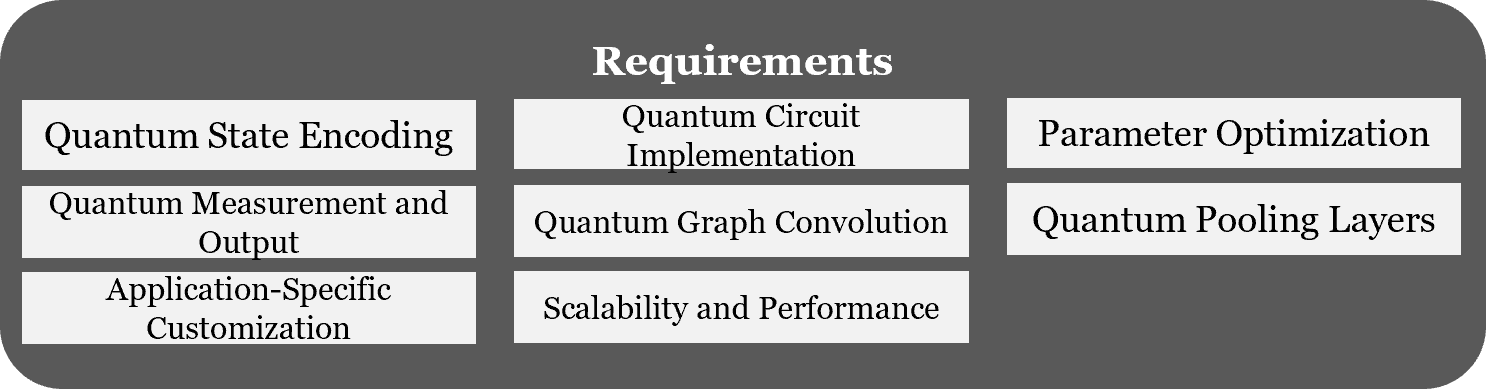
\includegraphics[width=\textwidth]{requirements.png}
    \caption[Identified requirements from the requirement analysis]{\label{img:requirements}{Identified requirements from the requirement analysis}}
    \end{figure} 
\label{subsec:requirements}
\subsection{Development of the QGNN}
\label{subsec:qgnndevelopment}

\section{Conclusion}
